% !TEX TS-program = pdflatex
% !TEX encoding = UTF-8 Unicode
\documentclass[a4paper]{article}
\usepackage[utf8]{inputenc}

%%% PAGE DIMENSIONS ------------------------------------------------------------
\usepackage{geometry}
\usepackage[parfill]{parskip}

%%% HEADERS & FOOTERS ----------------------------------------------------------
\usepackage{fancyhdr}
\pagestyle{fancy}

%%% PACKAGES -------------------------------------------------------------------
%\usepackage{morefloats}
\usepackage[hypcap=false,
	font=small,
	labelfont=bf,
	textfont=it]{caption}
\usepackage[pdftex]{graphicx}
\usepackage{tabu}
\usepackage{booktabs}
\usepackage{array}
\usepackage{enumitem}
\usepackage{longtable}
\usepackage{listings}
\usepackage{color}
\usepackage{pdflscape}
\usepackage[percentage]{overpic}
\usepackage{pdfpages}
\usepackage{tikz}
\usetikzlibrary{patterns}
% \usepackage[%
% 	activate={true,nocompatibility},
% 	final,
% 	tracking=true,
% 	kerning=true,
% 	spacing=true,
% 	factor=1100,
% 	stretch=10,
% 	shrink=10]{microtype}
% \microtypecontext{spacing=nonfrench}

%% BIBIOGRAPHY -----------------------------------------------------------------
\usepackage{cite}

%%% ToC (table of contents) APPEARANCE -----------------------------------------
% \usepackage[nottoc,notlof,notlot]{tocbibind}
% \renewcommand{\cftsecfont}{\rmfamily\mdseries\upshape}
% \renewcommand{\cftsecpagefont}{\rmfamily\mdseries\upshape}
\setcounter{tocdepth}{2}

\setlength\LTleft{0pt}
\setlength\LTright{0pt}

%%% PDF LINKS AND STYLE --------------------------------------------------------
% \usepackage[unicode=true,
% 	bookmarks=true,bookmarksnumbered=true,bookmarksopen=true,
% 	bookmarksopenlevel=2, breaklinks=false,pdfborder={0 0 0},backref=false,
% 	colorlinks=false]{hyperref}
\usepackage[bookmarks=true]{hyperref}
\hypersetup{%
	colorlinks=true,       % false: boxed links; true: colored links
	linkcolor=red,          % color of internal links (change box color with linkbordercolor)
	citecolor=green,        % color of links to bibliography
	filecolor=magenta,      % color of file links
	urlcolor=cyan           % color of external links
}

\newcommand\tablepage{%
	\newgeometry{
		top=1in,
		bottom=1.5in,
		left=3cm,
		right=3cm}
}
%%% END Article customizations

%*******************************************************************************
%******************************** END HEADER ***********************************
%*******************************************************************************

\begin{document}

%!TEX root = mainfile.tex
\begin{titlepage}
	\begin{center}
	\vspace*{\fill}

	\centering
	
\includegraphics[scale=1.0]{Logo.pdf}
	\vfill

	\hrule
	{\LARGE\bf Software Workshop 2 \\
		--- \\
		Real Time Multi-User Quiz System\\[0.4cm]}
	\hrule

	\vfill
	% \large
	% School of Computer Science\\
	% University of Birmingham

	\vfill
		Benjamin Crispin,\\
		Samuel Farmer,\\
		Deedar Fatima,\\
		Rowan Stringer,\\
		Josh Wainwright
	\vfill
		\textbf{Group Osaka}
	\vfill

	\vfill
	\textit{Supervisor:} Joe Gardiner \\
	\vfill
	\textit{Date:} March 2014
	\vfill
	\vfill

	\end{center}
\end{titlepage}

%\thispagestyle{empty}
%\vspace*{\fill}
%\noindent
%\begin{tabular}{ll}
%\end{tabular}

%\cleardoublepage
%\cleardoublepage


\tableofcontents
\addcontentsline{toc}{section}{Contents}
\newpage

\nocite{*}
\section{Protocol}
\label{sec:protocol}

The protocol for communicating between the different parts of the system is
based around objects. There exists an object class that can be created for any
of the several message types that could be needed to transfer information from
the server to the client, or from the client to the server. Each of these
objects implements the \texttt{Serializable} interface, allowing them to be
converted to bytes and transfered across the socket connection using object
streams.

\begin{description}
	\item[AnswerResponse object] \hfill \\ To respond to a question, the
		Student selects the desired option. This information is passed to the
		server using an AnswerResponse object which simply holds the response
		and the timestamp to indicate when they made the selection.

	\item[DisplayQuestion object]\hfill \\ In order to signify that the
		allotted time for the current question has ended, and the next question
		should be displayed, the server sends a DisplayQuestion object to all
		of the clients and they should move on to the next question in the Quiz
		object and change the GUI accordingly.

	\item[LoginReply object]\hfill \\ Once a loginRequest has been received by
		the server, a LoginReply will be sent back. This gives the client the
		information about the requested login, most importantly if the login
		was successful, as well as the type of user that made the login,
		Student or Admin. This information is used to display the correct user
		interface.

	\item[LoginRequest object]\hfill \\ This is the first object that could be
		created.  It is sent, by the client, to the server and contains the
		username of the Student that is attempting to login and the
		\texttt{java.lang.String} hash code of the inserted password. Though
		the security concerns of such a trivial system are non-existent, the
		password is never stored in plaintext.

	\item[Question object]\hfill \\ There exist several question objects in
		each Quiz object. They store the information required to present a
		Student with a question and the possible answers. Again, there is very
		little functionality as the question only serves as a wrapper for the
		question text and the possible answers that the user could respond
		with.

	\item[Quiz object]\hfill \\ This is the most important object. It has very
		little functionality, simply acting as a wrapper to hold and easily
		transfer several Question objects.

	\item[QuizRequest object]\hfill \\

	\item[Score object]\hfill \\ When the quiz has been completed, each of the
		clients will display the position of it's user relative to the other
		Students. This object contains the score of all of the users so that
		each of the clients can work out where they are in the ranking.

	\item[StartQuiz object]\hfill \\ Once the user has successfully logged into
		the system, the next major event is the start of the quiz. This is
		signaled by an Admin user who is connected to the server, this
		information must then be relayed to each of the connected clients. A
		StartQuiz object is sent to each of the clients, who, on receiving it,
		will display the first question to the user.
\end{description}

\section{Client}
\label{sec:client}

The client exists to accept messages sent by the server, and present them in an
order and a format that the user interface can present to the user, as well as
accept the information entered by the user into the user interface and pass it
to the server.

\subsection{System Design}
\label{sub:client_system_design}

\begin{enumerate}

	\item \textbf{Login}

	When a client is started, a \texttt{QuizClient} object is created and
	starts the main loop. The initial stages set up the connection with the
	server and waits for the user to login. When the user enters their
	information, a \texttt{LoginRequest} object is created and pass to the
	server containing the username and password, to be checked against the
	contents of the database. The client then waits for a reponse from the
	server to indicate if the login was successfull or not. This comes in the
	form of a \texttt{LoginReply} object. If this says that the login was
	unsuccessful, the user is asked to re-input their details, otherwise, the
	display is changed and the options screen is shown.

	\item \textbf{Student/Admin}

	There exists separate functionality withing the client depending on if the
	user is a Student user, i.e.\ going to be answering questions, or an Admin,
	i.e.\ the teacher who starts and moderates the quiz. Distinguishing between
	these two is done by the server by checking the details associated with
	that user in the database. The \texttt{LoginReply} object contains this
	information and the client can then display the correct interface depending
	on the type of user that logged in.

	\item \textbf{Client Listens from Server}

	From here, the user can select the ``Start Quiz'' option to start the
	quiz. This causes the display to change to display the waiting screen and
	the client waits for information from the server.

	From this point on, the client waits for any object to be sent from the
	server and acts according to what that object was. The possible objects
	that the client now expects to be able to distinguish between are:
	\begin{itemize}
		\item \texttt{Quiz}
		\item \texttt{StartQuiz}
		\item \texttt{DisplayQuestion}
		\item \texttt{Score}
	\end{itemize}

	\begin{description}
		\item[\texttt{Quiz}]\hfill \\ This object contains the information
		about the quiz itself, the number of questions, their contents and the
		duration that each question should be displayed for. It should only
		ever be recieved once by the client, at the start of the session,
		reducing the transfer of information over the connection.

		\item[\texttt{StartQuiz}]\hfill \\ Once an Admin has logged in, they
		have control over the start of the quiz. When they decide to start the
		quiz, this object is sent to each of the listening clients and so the
		client will procede to show the first question from the \texttt{Quiz}
		object.

		\item[\texttt{DisplayQuestion}]\hfill \\ The first question is
		displayed as soon as the \texttt{StartQuiz} object is recieved. After
		this point in the quiz, the questions are changed when this object is
		received. The value contained verifies which question is to be
		displayed.

		\item[\texttt{Score}]\hfill \\ After each question has been answered,
		the client can display a leader board showing the score of all the
		clients that have so far answered the current question along with the
		current client's position in this list. This object tells the client
		the relevant information for displaying the scores of the other
		clients.
	\end{description}

	\item \textbf{Sent by Client}

	There are also a number of objects that the client can create and send to
	the server at different stages of the quiz:
	\begin{itemize}
		\item \texttt{LoginRequest}
		\item \texttt{QuizRequest}
		\item \texttt{AnswerResponse}
	\end{itemize}

	\begin{description}
		\item[\texttt{QuizRequest}]\hfill \\ This is sent by the client when an
		Admin is logged in in order to request a particular quiz from the
		server. Since the server can hold many quizzes, each with their own set
		of questions and answers, the Admin has the option to choose which of
		these to play when they log in.

		\item[\texttt{AnswerResponse}]\hfill \\ This is the object that tells
		the server what answer the Student gave. It contains their response, so
		that it can be logged in the database, and the time it took for the
		Student to make their selection.
	\end{description}

\end{enumerate}

\section{Server}
\label{sec:server}

The server exists to create a link between the database and the quiz program,
as well creating connections with, and processing requests from, clients.

\subsection{System Design}
\label{sub:system_design}

\begin{enumerate}
	\item \textbf{Initialising the server}

	When the server starts, a \texttt{QuizServer} object is created. The object
	creates a connection with the database by taking advantage of the inbuilt 
        Java Database Connectivity (JDBC) functionality, which allows the server 
        object to retrieve, and update, information contained in the database. In 
        addition to this, a \texttt{ServerSocket} object is created, which waits to
        receive connections from \texttt{QuizClient} objects. When a connection from 
        a client is received, a new \texttt{ClientThread} object is created.

	\item \textbf{Database Connectivity}

	The server interacts with the database through static methods contained in
	the \texttt{QuizJDBC} class.  The class allows the server to establish a
	connection with the database through a \texttt{getConnection} method, which
	returns a Connection object.

	A second method, \texttt{isUser}, is called by the server when it receives
	a \texttt{LoginRequest} object from a client thread. The method returns a
	\texttt{LoginReply} object containing the results of the query, which is
	sent to the client.

	The final method, \texttt{getQuiz}, is called when the server receives a
	\texttt{QuizRequest} object from a client, and returns a \texttt{Quiz}
	object.

	\item \textbf{\texttt{ClientThread} Objects}

	When the server establishes a connection with a client, a
	\texttt{ClientThread} object is created, spawning a thread which allows
	interactions to occur between the server and  client. The server then waits
	to receive a \texttt{LoginRequest} from the client, and returns a
	\texttt{LoginReply} object upon receiving it.  Once the client has logged in,
	the server distinguishes between Student and Admin users.

	\item \textbf{Admin Clients}

	If a connection to an Admin has been made, the server waits for a
	\texttt{QuizRequest} object. Once received, the server retrieves the quiz
        in the database through the \texttt{QuizJDBC} class, then distributes this 
        to all connected Student clients.

	\item \textbf{Student Client}

	If a student user has logged in, their instance of \texttt{ClientThread} 
        on the server will wait until the Quiz has been set to ready by an admin. 
        Once a quiz has been started, the server sends the \texttt{Quiz} object to
	all connected student clients, and then waits to receive an \texttt{AnswerReponse}
	from each of the Student client threads. The \texttt{AnswerReposnse} objects 
        contain the clients response to a question, and the time that it took for 
        them to answer it.  The server than calculates the clients score,
	and the results are stored in an ArrayList, which contains the results of
	all connected Student clients.  This ArrayList of scores is sent to
	the connected clients every time it is updated, allowing users to see an
        'updating' results table which contains all student clients scores.

        \item \textbf{Quiz Time}
         
        In order to carry out admin tasks on the server without disrupting the
        main thread which is listening for connecting clients, an inner class
        \texttt{QuizTime} which extends Thread was created. The thread loops through 
        during the quiz session, checking certain conditions, to which it 
        should respond with specific tasks. For example, it checks whether no 
        clients are connected, in which case the quiz stops. It also checks 
        whether the first question of the quiz has finished being asked, in 
        which case further student clients should not be allowed to join the
        quiz.
        
    
        

\end{enumerate}

\section{Database}
\label{sec:database}



\section{Team Organisation}
\label{sec:team_organisation}

The group consists of 5 students. Since there were a number of distinct
sections to the project, the different components were distributed among the
members of the team with one person in a position of responsibility for that
component and another to help. The allocations were as follows.

\begin{table}[htbp]
	\centering
	\begin{tabular}{@{}rll@{}}
		\toprule
\textbf{Component} & \textbf{Responsible} & \textbf{Assiting} \\ \midrule
		GUI              & Benjamin Crispin & Deedar Fatima    \\
		Client           & Josh Wainwright  & Rowan Stringer   \\
		Server           & Rowan Stringer   & Benjamin Crispin \\
		Database         & Deedar Fatima    & Sam Farmer       \\
		Protocol         & Sam Farmer       & Josh Wainwright  \\
		\bottomrule
	\end{tabular}
\end{table}

These roles were followed closely during the initial stages of development and
through the first round of testing. As the program became more complete and bug
fixes were required, the roles were shared more evenly through the team. This
has the advantage that all members have a full understanding of all aspects of
the project having worked on all parts at some time.

\tablepage%
\begin{landscape}

\section{Test Plan}
\label{sec:test_plan}

\renewcommand{\arraystretch}{1.3}
\begin{longtabu}{c l X c c}
\toprule
S.No & Category & Description & Expected Result & Actual Result \\
\midrule
1 & Registration & User is able to register by providing first name, last name,
username and password. & & \\

2 & Registration & System should display username and password guidelines to
users. & & \\

3 & Registration & System validates the credentials; dispays an error message
if user provides invalid username and password and asks user to choose valid
credentials. & & \\

4 & Registration & If user enters valid credentials, system checks if the
entered credentials already exists in the the users table. If credentials
exists, system asks the user to choose different credentials. & & \\

5 & Registration & System inserts the credentials in the users table if the
user enters valid credentials. A unique ID is created for the user in users
table. & & \\

6 & Login & System displays the login page where user can enter username and
password and login to the system. & & \\

7 & Login & System checks the entered credentials in the users table; displays
an error message if incorrect credentials are entered and asks user to re-enter
credentials. & & \\

8 & Login & If correct credentials are entered, user is taken to the Home page.
& & \\

9 & HomePage-Student & Student homepage should display the buttons – Start,
View Result, Update Profile and Quiz rules. & & \\

10 & HomePage-Student & Quiz should start when Student clicks on ``Start''
button. & & \\

11 & HomePage-Student & Quiz result should be displayed when Student clicks on
``View Result'' button. What is shown in View Result page? & & \\

12 & HomePage-Student & Profile page should be displayed when Student clicks on
``Update Profile'' button. User should be able to edit profile; save changes or
cancel changes. & & \\

13 & HomePage-Student & Quiz rules should be displayed when stuent clicks on
``Quiz Rules'' button. A new window or a popup screen? & & \\

14 & HomePage-Admin & Admin homepage should display the buttons – Start, View
Result, Question settings (Add, remove or update questions), Update Profile.
(Check the options displayed). & & \\

15 & HomePage-Admin & Admin should be able to select a quiz and click on Start
to start the quiz. & & \\

16 & HomePage-Admin & Quiz result should be displayed when Admin clicks on
``View Result'' button. What is shown in View Result page? & & \\

17 & HomePage-Admin & Admin should be able to add, remove or update
questions/answers in questions table in the Question settings page. & & \\

18 & HomePage-Admin & Profile page should be displayed when Admin clicks on
``Update Profile'' button. Admin should be able to edit profile; save changes or
cancel changes. & & \\

19 & Play Quiz-Student & The quiz name should be displayed in quiz page. & & \\

20 & Play Quiz-Student & Each quiz consists of 10 questions. & & \\

21 & Play Quiz-Student & Each question has a set of possible answers (maximum
4). & & \\

23 & Play Quiz-Student & Timer is displayed when question appears on screen. &
& \\

24 & Play Quiz-Student & Student is able to choose an answer by clicking on the
answer. & & \\

25 & Play Quiz-Student & When a Student chooses the correct answer before time
runs out, timer stops. The other Students should not be able to select an
option once the timer stops. & & \\

26 & Play Quiz-Student & After quiz finishes, the result is inserted into
user\_result table. & & \\

27 & Play Quiz-Student & Student should be able to see feedback after quiz
finishes. & & \\

28 & Play Quiz-Student & Student should be able to view result after quiz
finishes (and after answering a question?). & & \\

29 & Play Quiz-Student & Student should b able to view the historical result
data from user\_result table after quiz finishes. & & \\

30 & Play Quiz-Student & Student should be able to click on the close buttom to
exit the quiz. & & \\

31 & Play Quiz-Admin & Admin should be able to click on start button to start
the quiz once all Students have logged in. & & \\

32 & Play Quiz-Admin & Admin should be able to see the result after each
question is answered. & & \\

33 & Play Quiz-Admin & Admin should be able to see the result summary after
quiz finishes. & & \\

34 & Play Quiz-Admin & Student should be able to click on the close buttom to
exit the quiz. & & \\

35 & Server-Client & System ensures that all clients and server are
synchronised. & & \\

36 & JDBC & Database connection is established from JDBC\@. & & \\
\bottomrule
\end{longtabu}
\end{landscape}
\restoregeometry%


\bibliographystyle{unsrt}
\bibliography{references}

\appendix

\addcontentsline{toc}{section}{Class Diagram}

\newgeometry{bottom=0in}
\thispagestyle{empty}
\begin{figure}[h!]
	\vspace{-2cm}
	\centering
	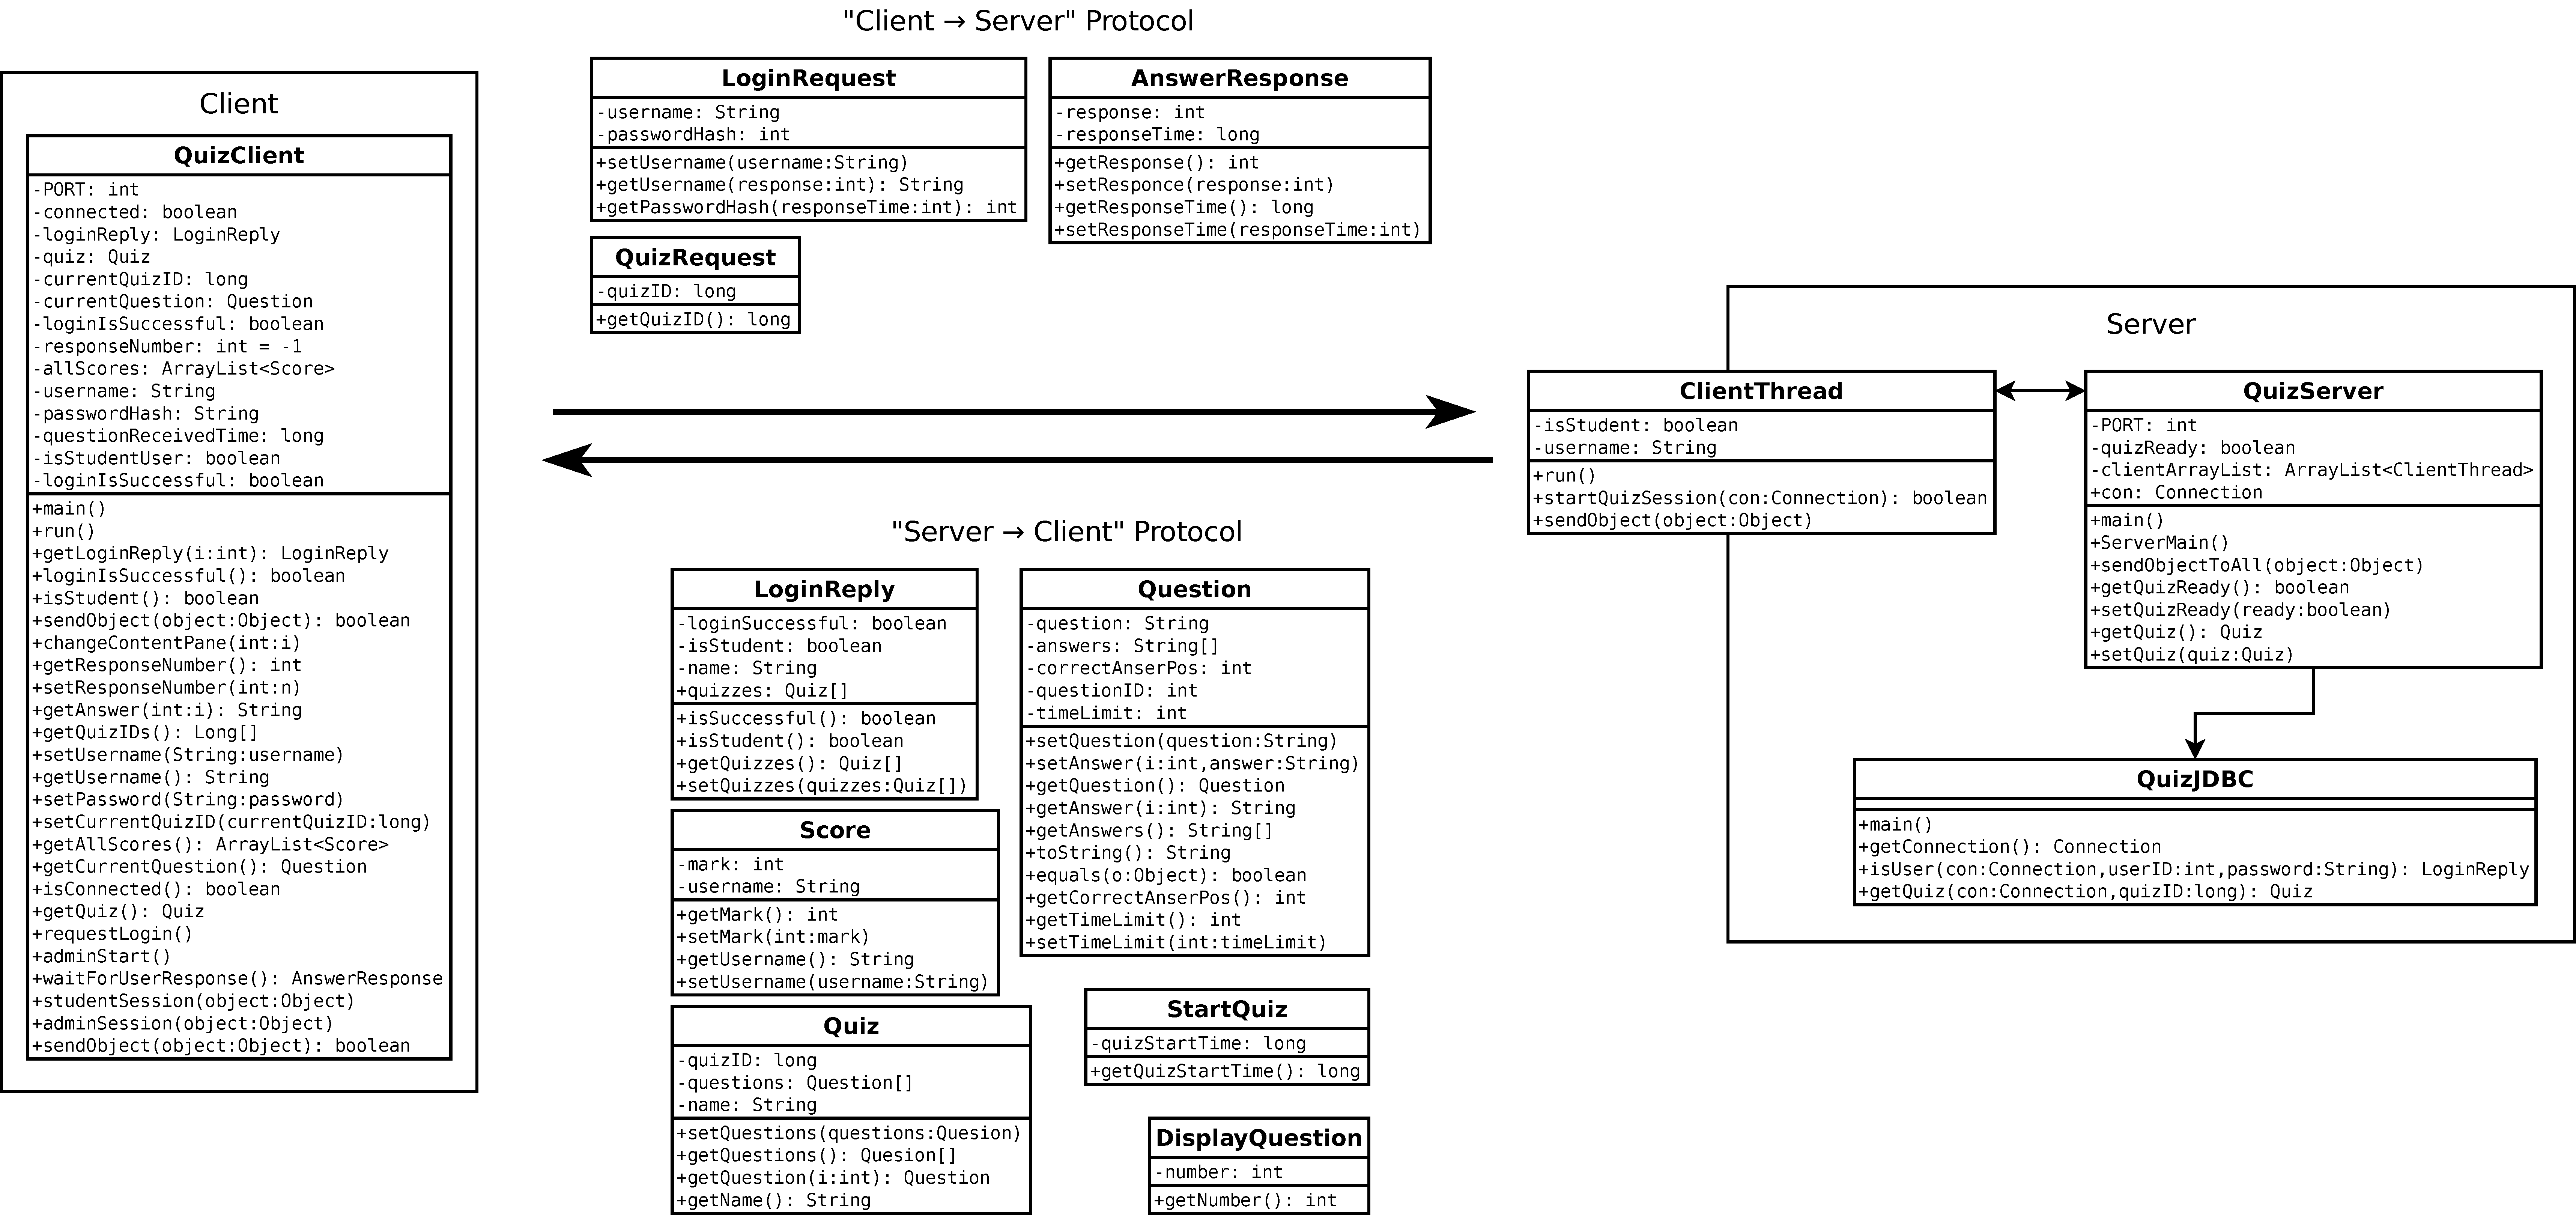
\includegraphics[angle=90,height=\textheight]{img/objectDiagram.pdf}
\end{figure}
\restoregeometry%

\addcontentsline{toc}{section}{Database Design}

\includepdf[pages=-]{img/Database_Design_Specification_v2.pdf}

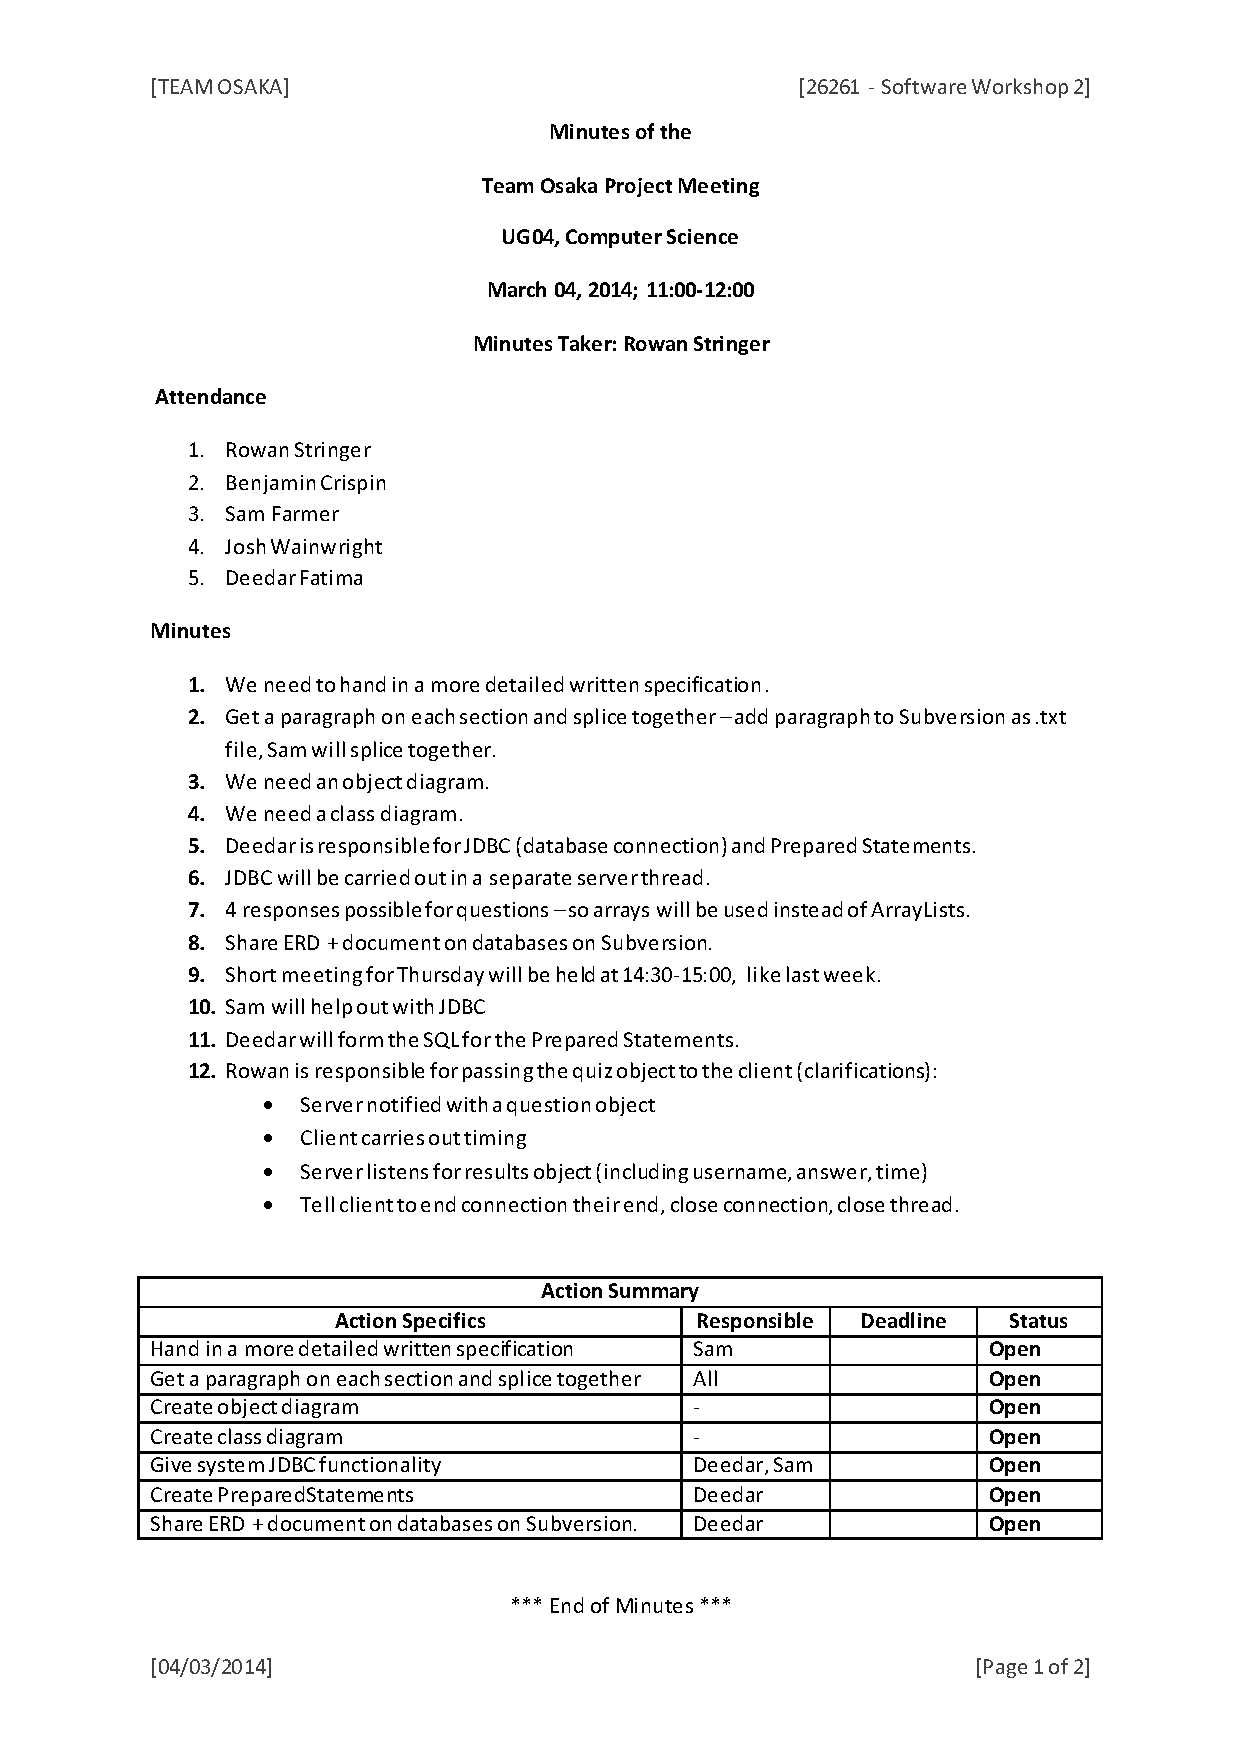
\includepdf[pages=-]{../MeetingMinutes/OSAKA_04032014_Minutes.pdf}
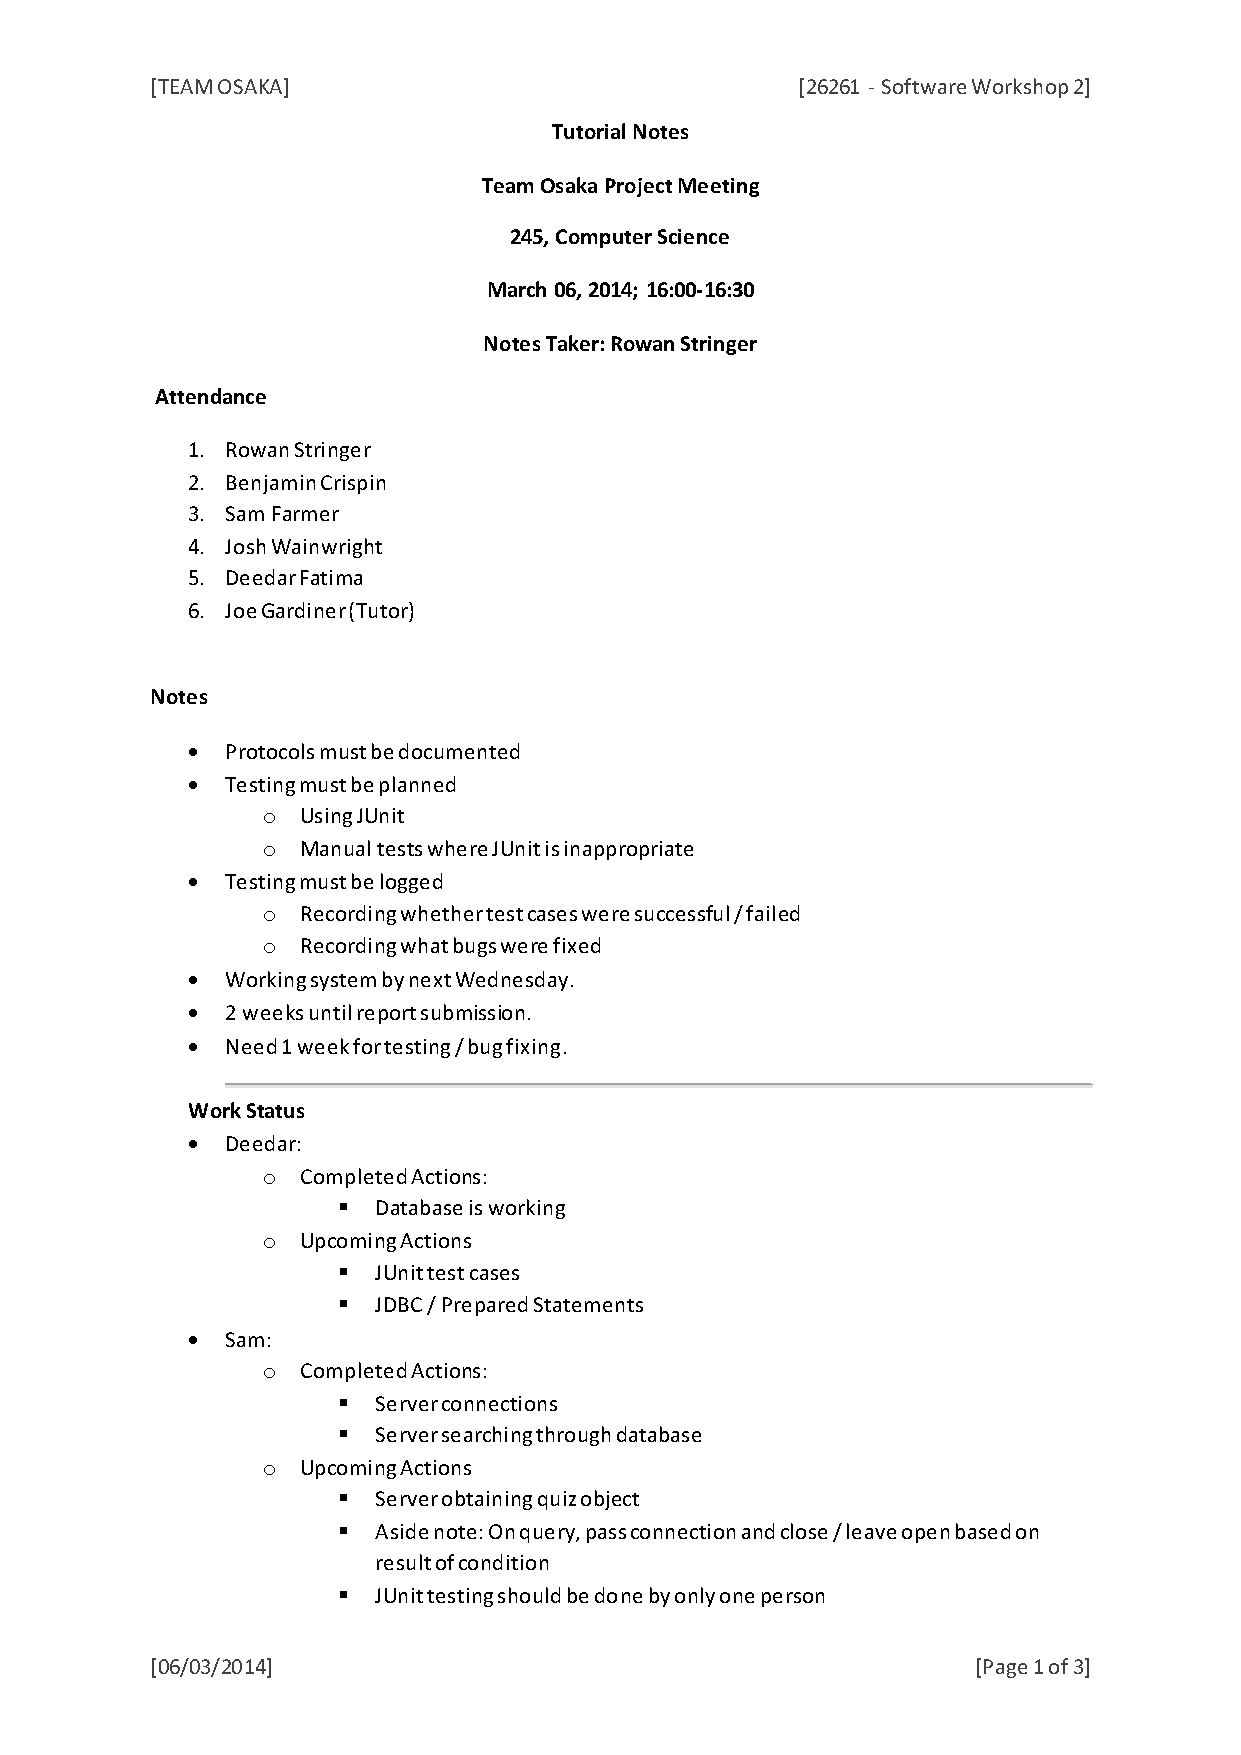
\includepdf[pages=-]{../MeetingMinutes/OSAKA_06032014_Tutorial_Notes.pdf}
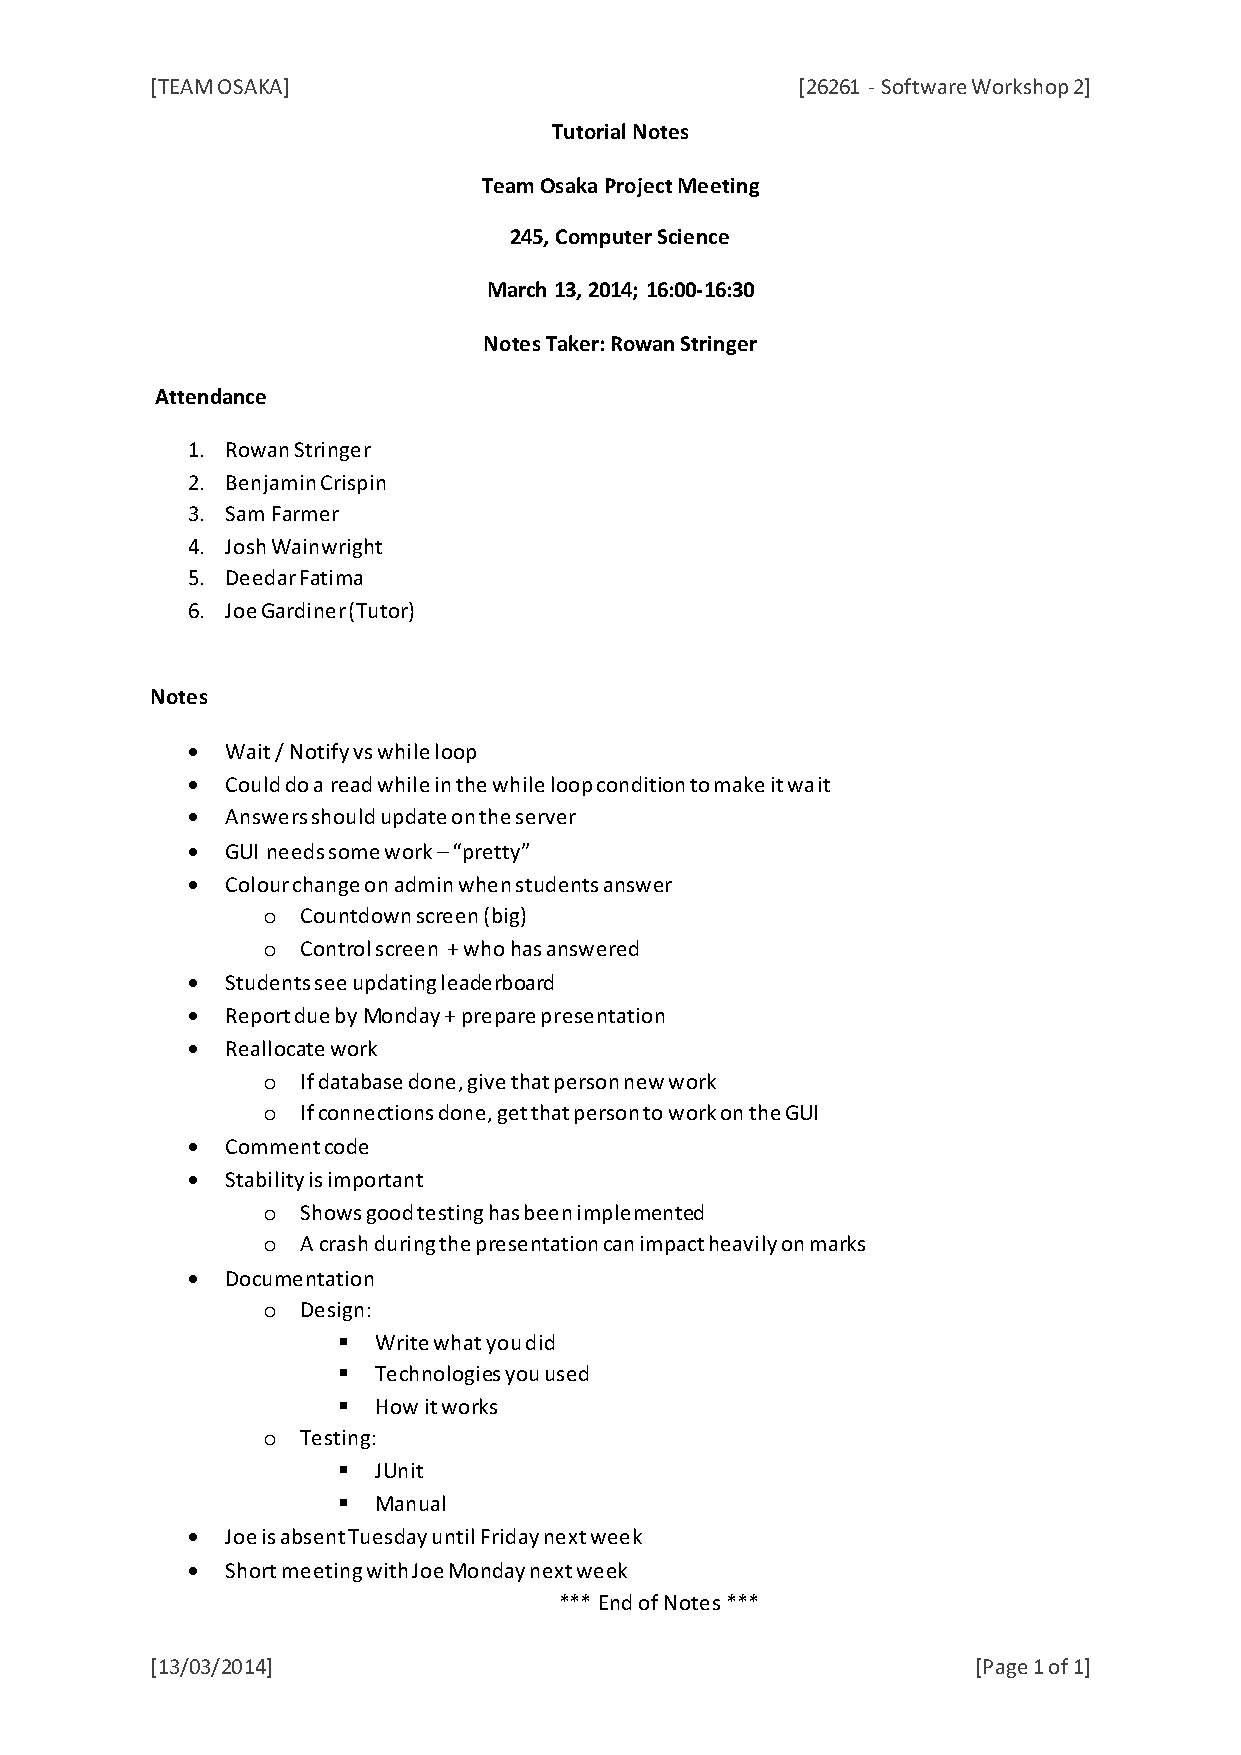
\includepdf[pages=-]{../MeetingMinutes/OSAKA_13032014_Tutorial_Notes.pdf}

\includepdf[pages=-]{../MeetingMinutes/OSAKA_21022014_Minutes.pdf}
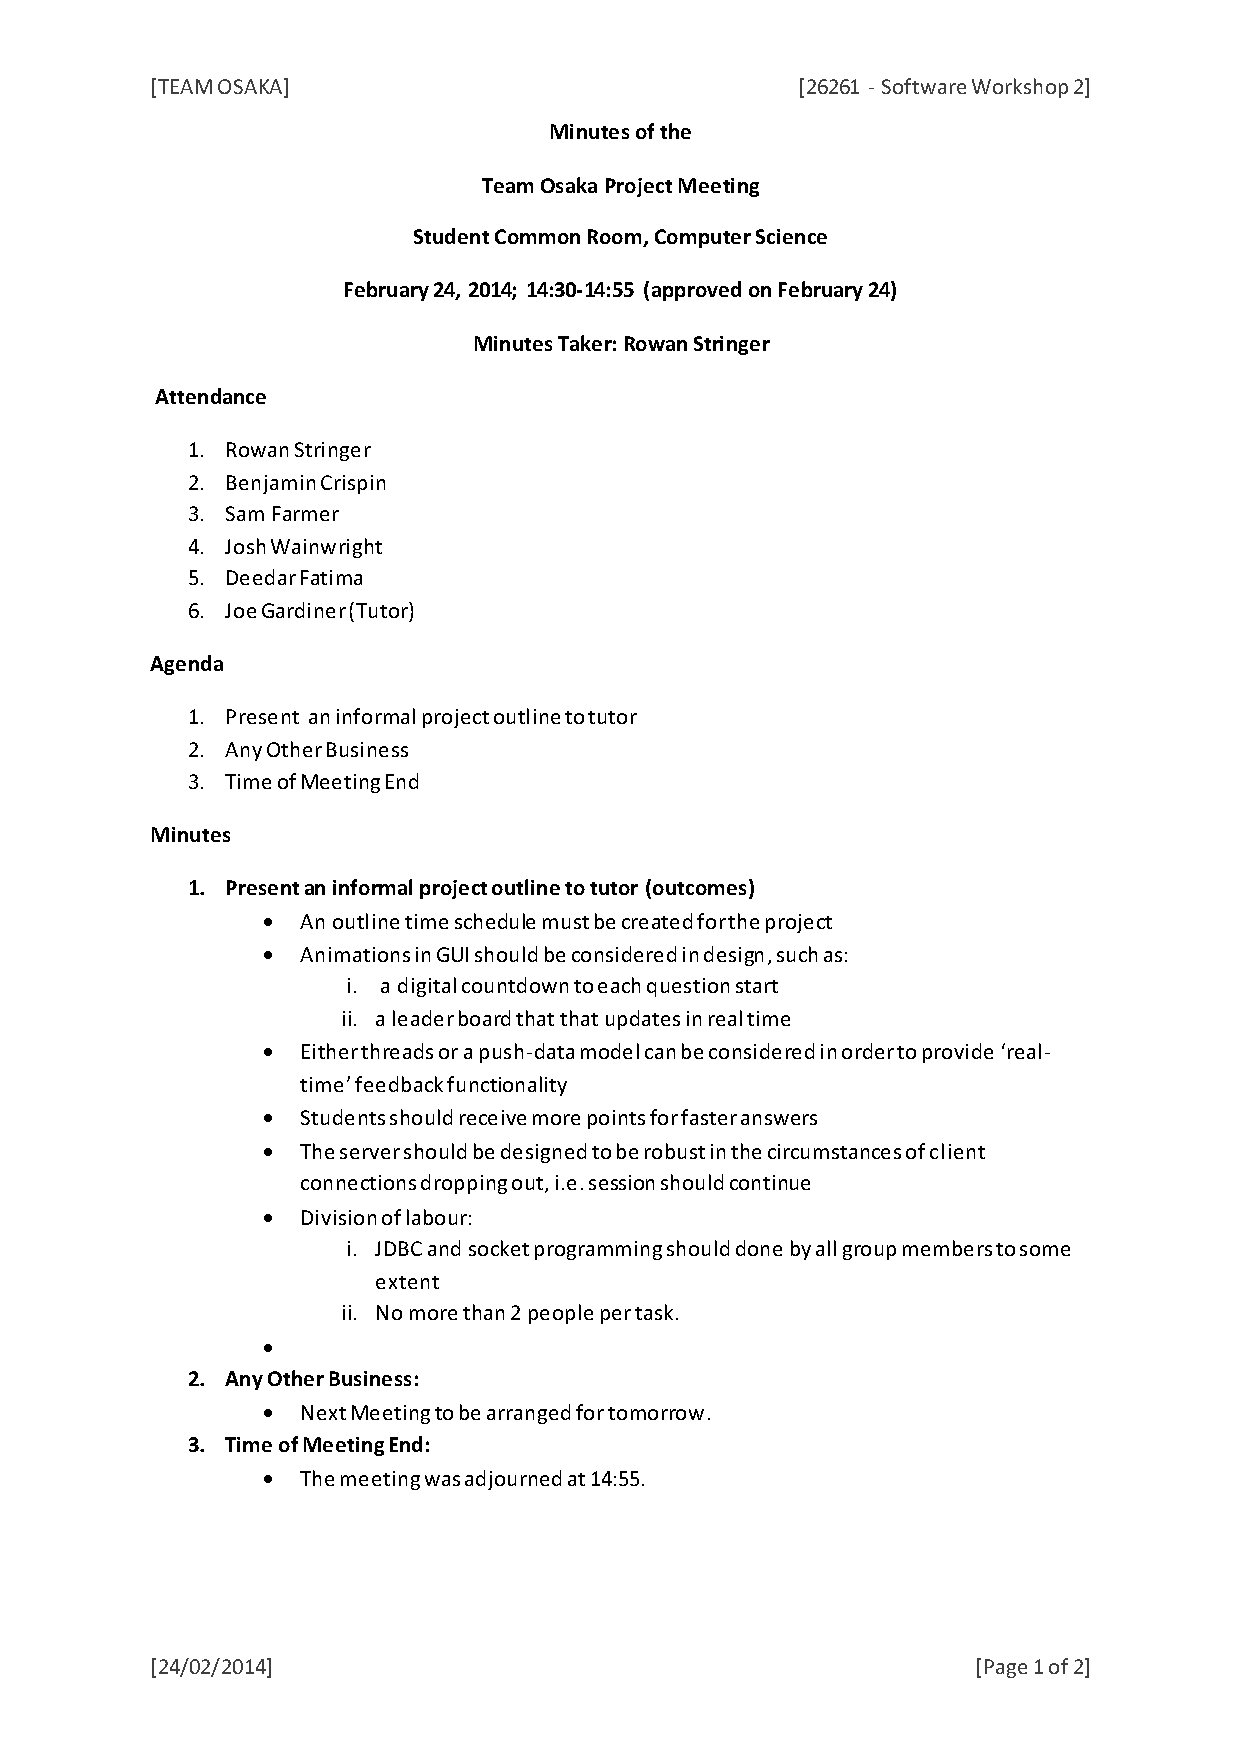
\includepdf[pages=-]{../MeetingMinutes/OSAKA_24022014_Minutes.pdf}
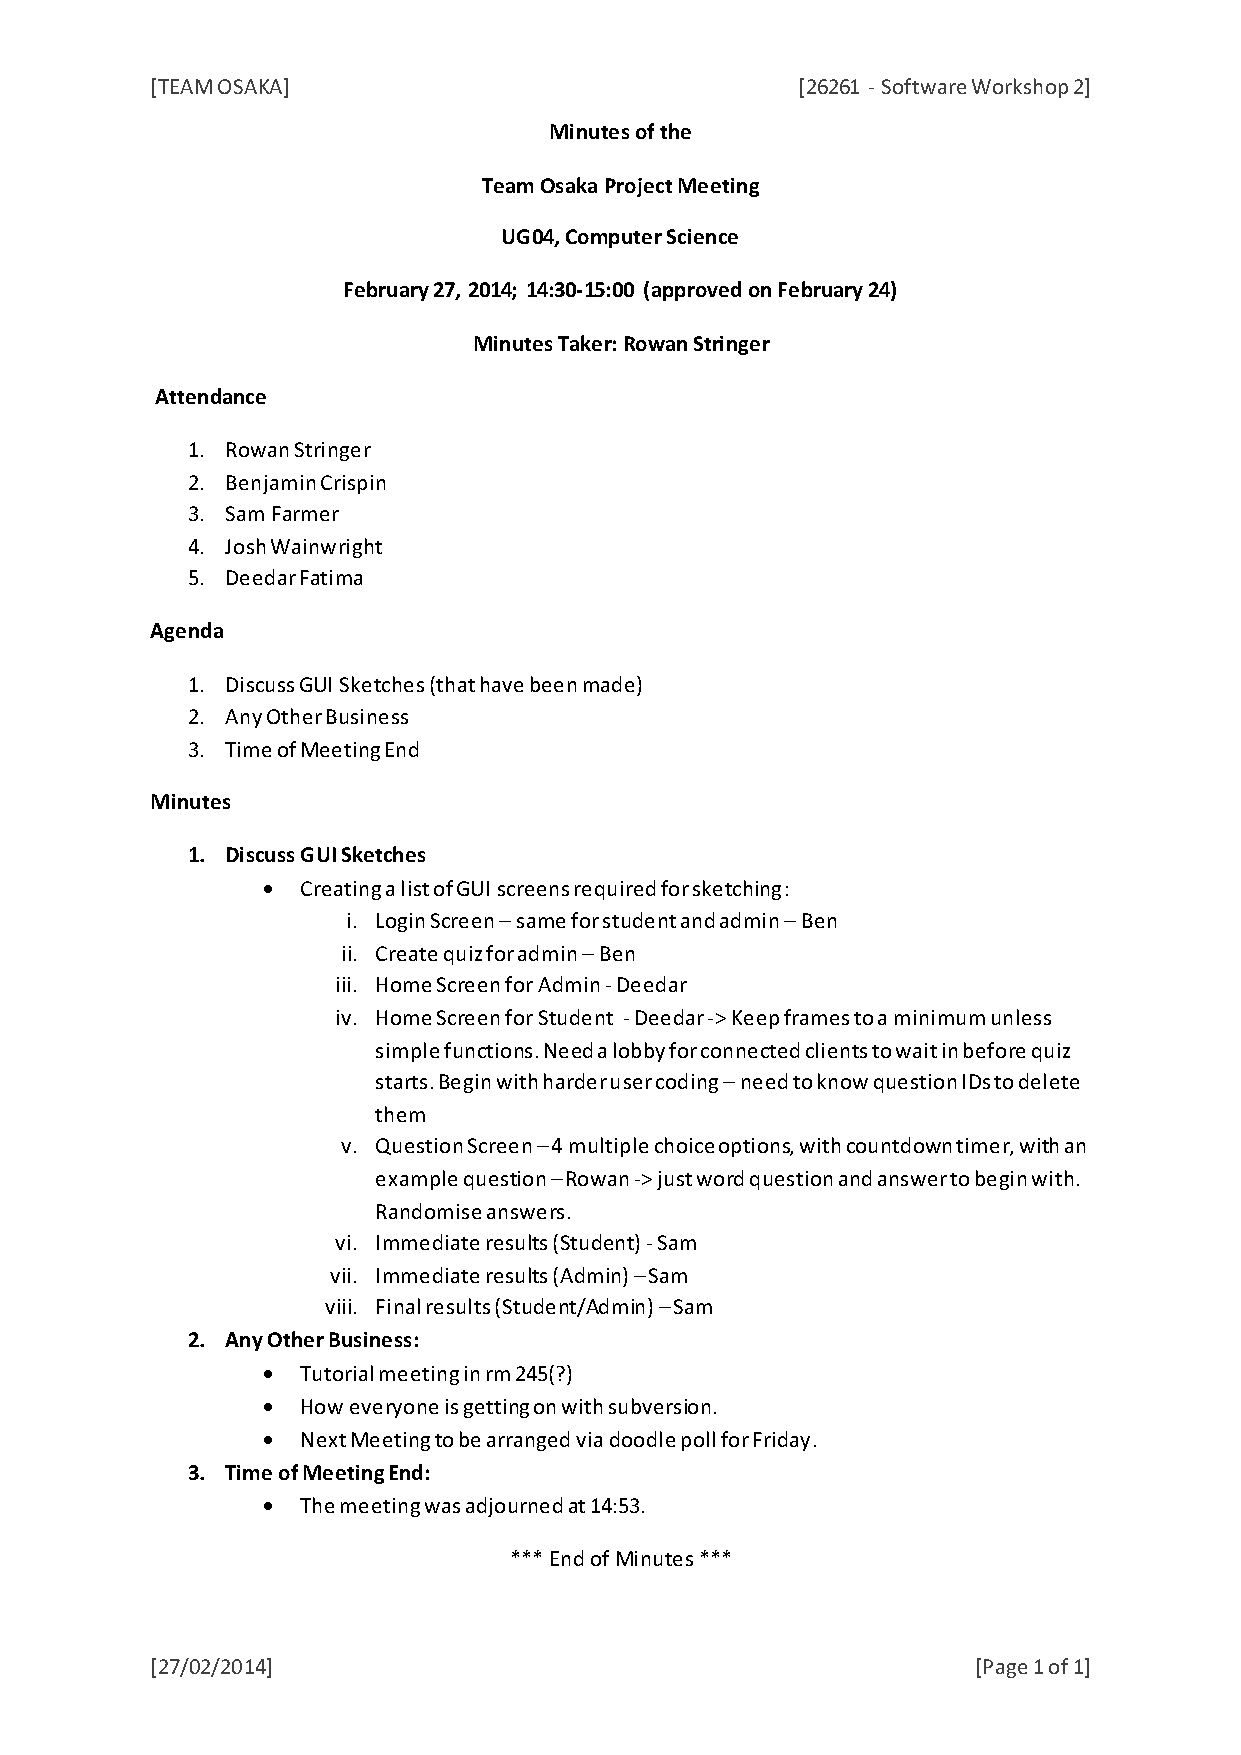
\includepdf[pages=-]{../MeetingMinutes/OSAKA_27022014_Minutes.pdf}
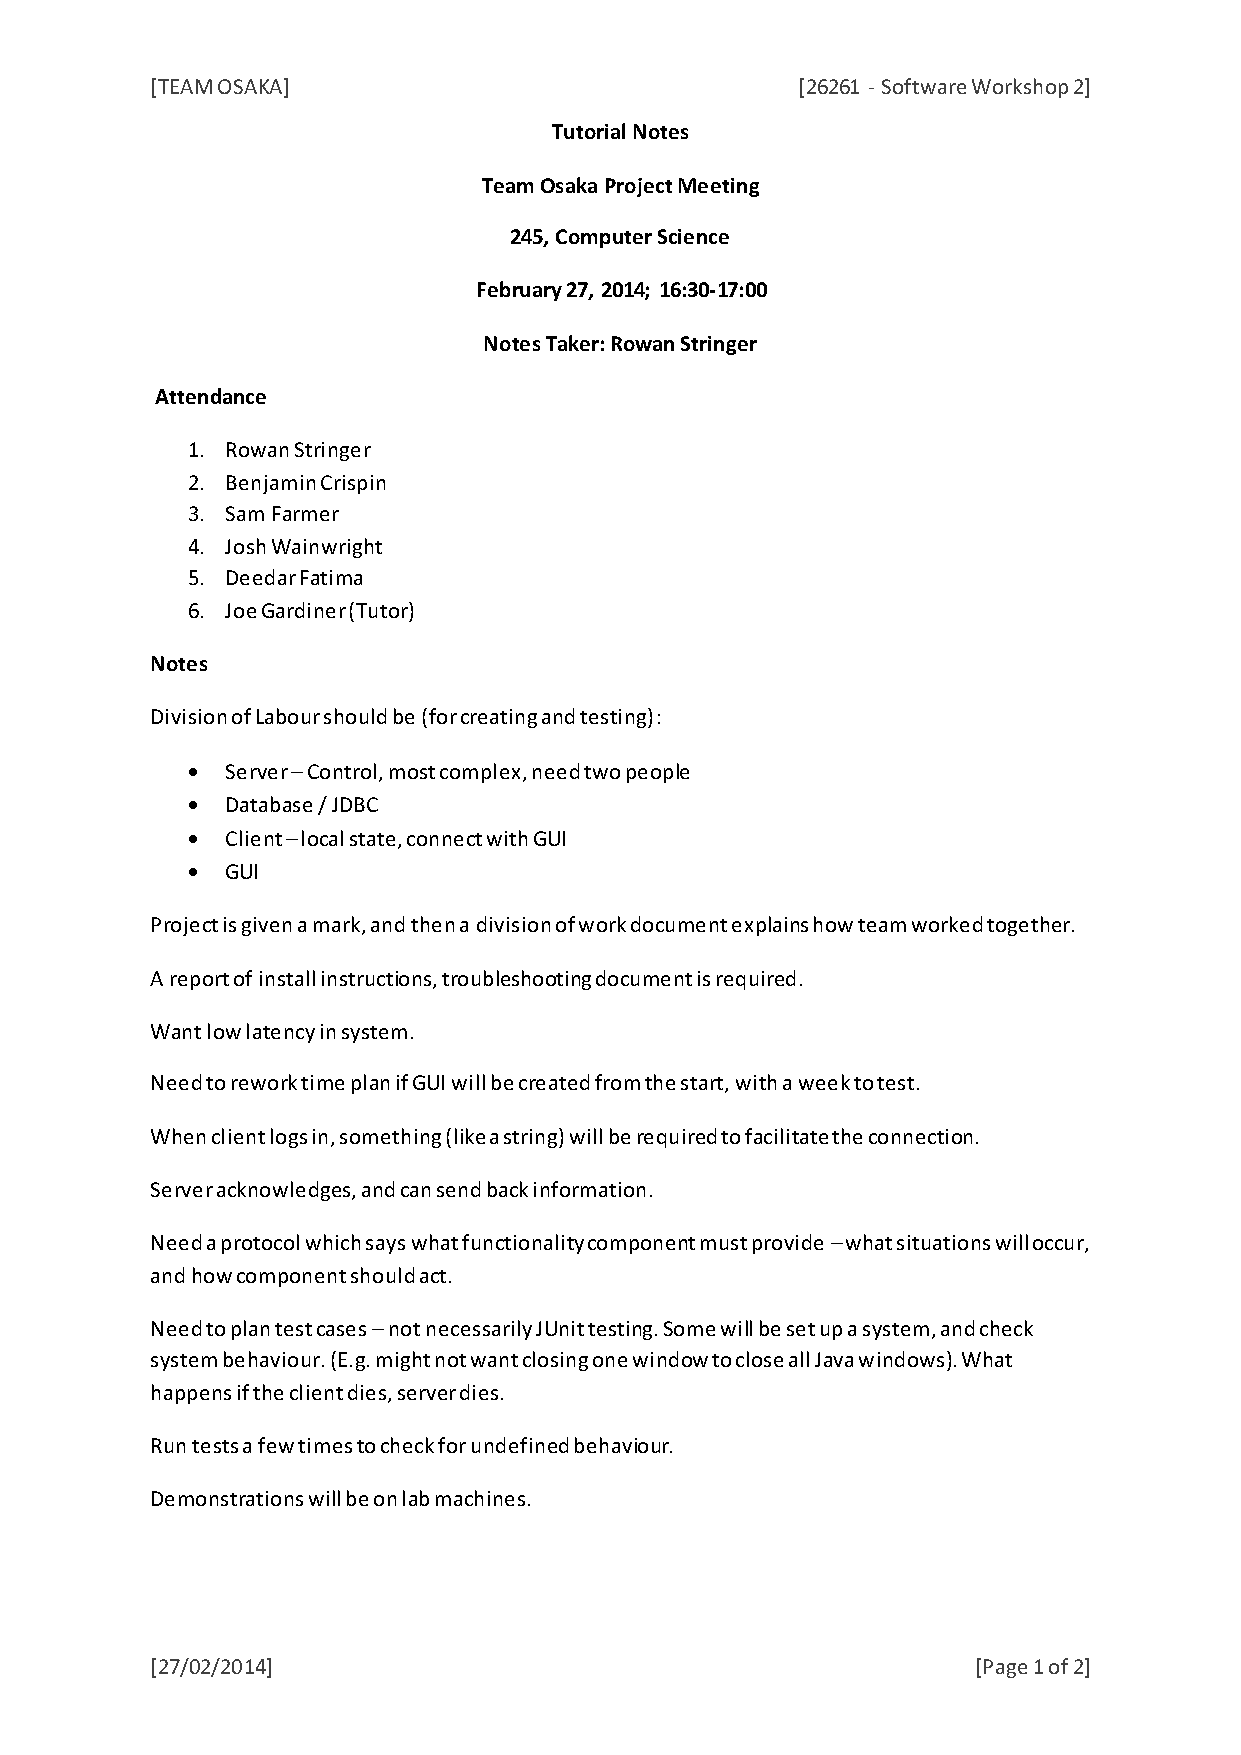
\includepdf[pages=-]{../MeetingMinutes/OSAKA_27022014_Tutorial_Notes.pdf}

\end{document}

% vim: autochdir
